\chapter{Escenarios}
    \label{chap:six}
    
\section{Ciudad 1. Cruce simple}
\begin{figure}[H]
    \centering
    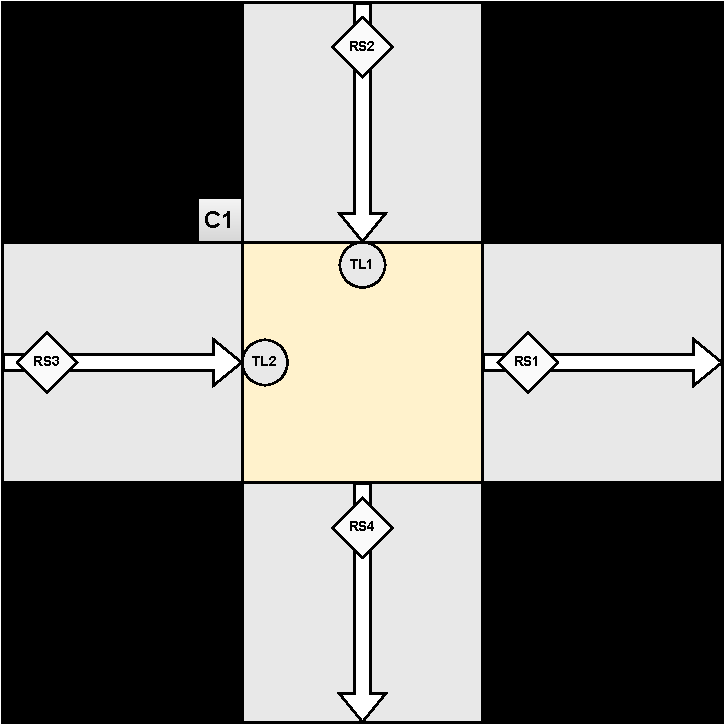
\includegraphics[width=1\linewidth]{text/image/DCruc-CSimple-Topologia.pdf}
    \caption{Topología del cruce simple}
    \label{fig:cruce_simple_topologia_esc}
\end{figure}

\newpage
\section{Ciudad 2. Matriz de cruces simples 2x1}
    \label{section:cruce_simple2x1}
\begin{figure}[H]
    \centering
    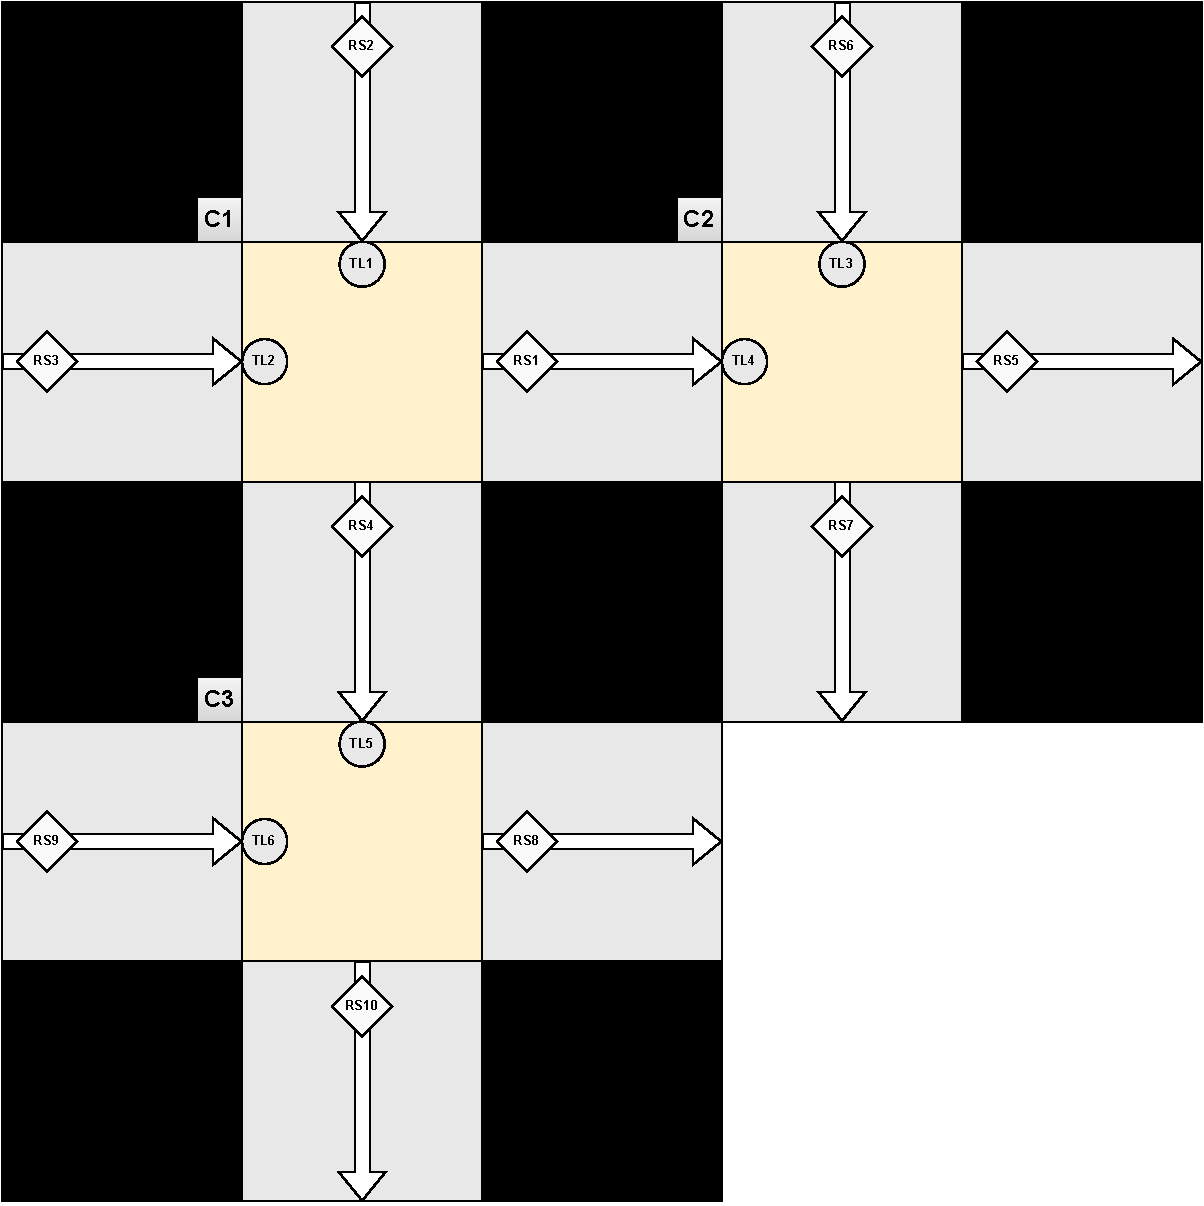
\includegraphics[width=1\linewidth]{text/image/DCruc-CSimple2x1-Topologia.pdf}
    \caption{Topología de la matriz de cruces simples 2x1}
    \label{fig:cruce_simple2x1_topologia}
\end{figure}

\newpage
\section{Ciudad 3. Matriz de cruces simples 2x2}
\begin{figure}[H]
    \centering
    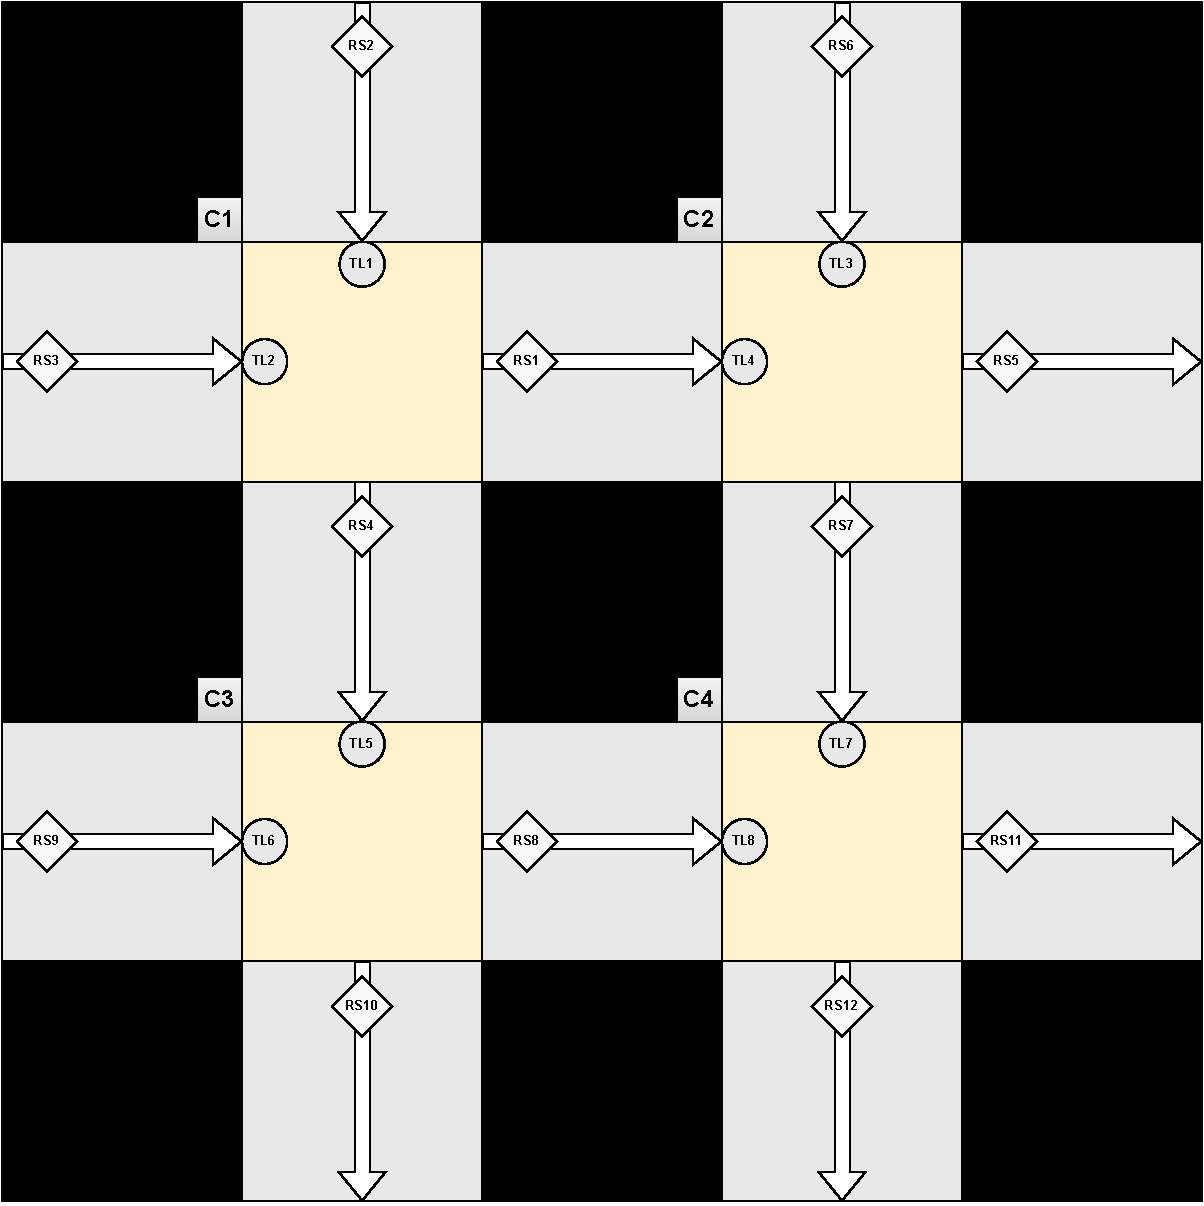
\includegraphics[width=1\linewidth]{text/image/DCruc-CSimple2x2-Topologia.pdf}
    \caption{Topología de la matriz de cruces simples 2x2}
    \label{fig:cruce_simple2x2_topologia}
\end{figure}

\newpage
\section{Ciudad 4. Matriz de cruces simples 3x3}
\begin{figure}[H]
    \centering
    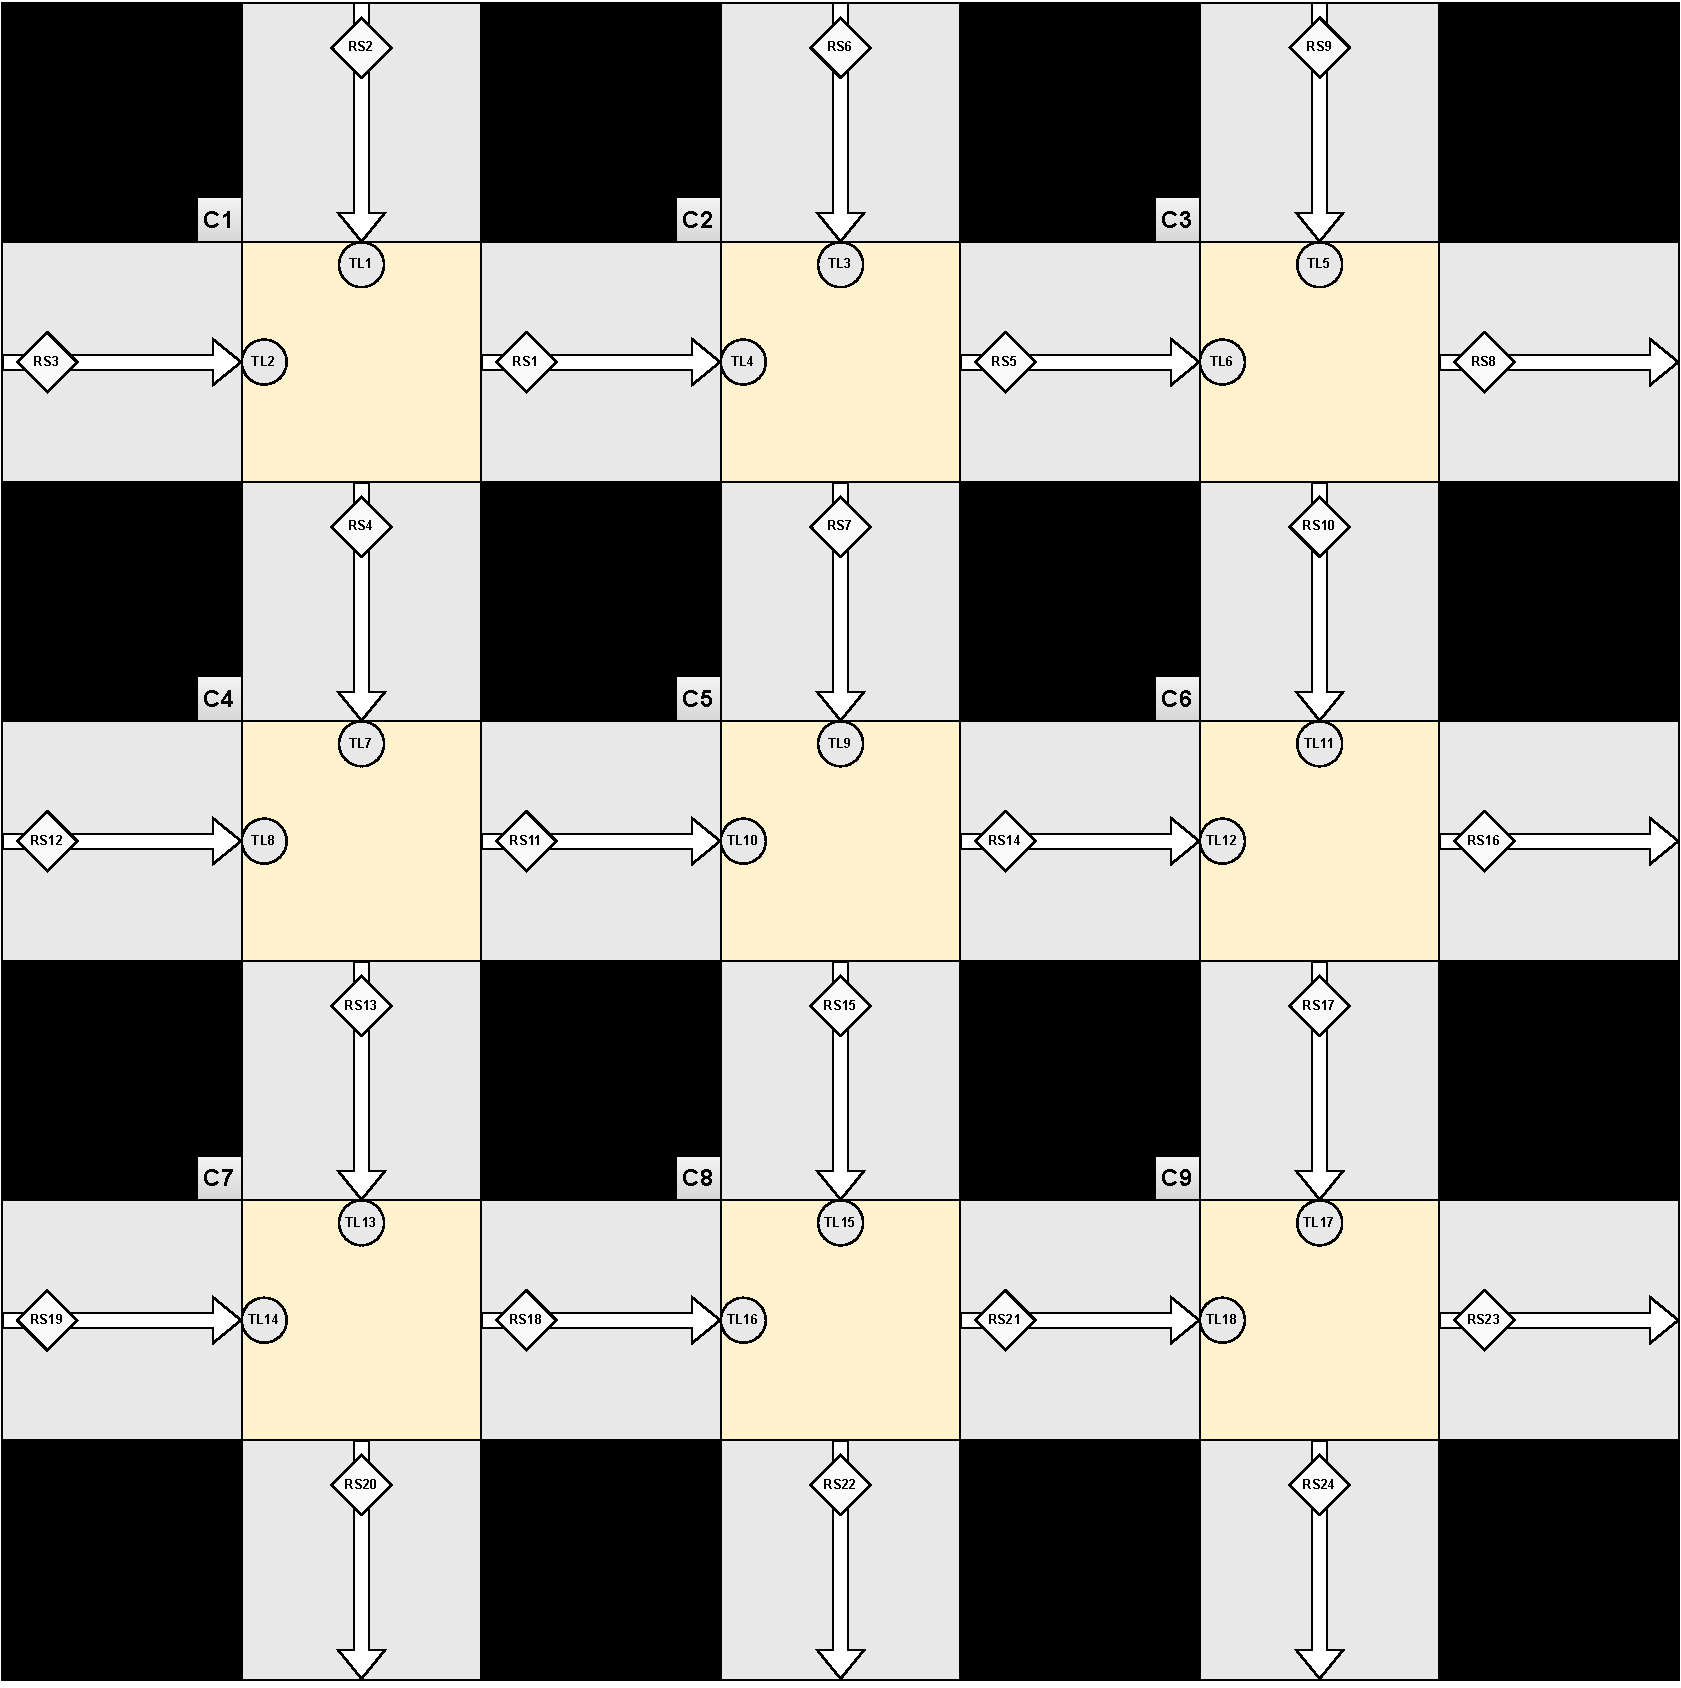
\includegraphics[width=1\linewidth]{text/image/DCruc-CSimple3x3-Topologia.pdf}
    \caption{Topología de la matriz de cruces simples 3x3}
    \label{fig:cruce_simple3x3_topologia}
\end{figure}

\newpage
\section{Ciudad 5. Cruce estándar}
\begin{figure}[H]
    \centering
    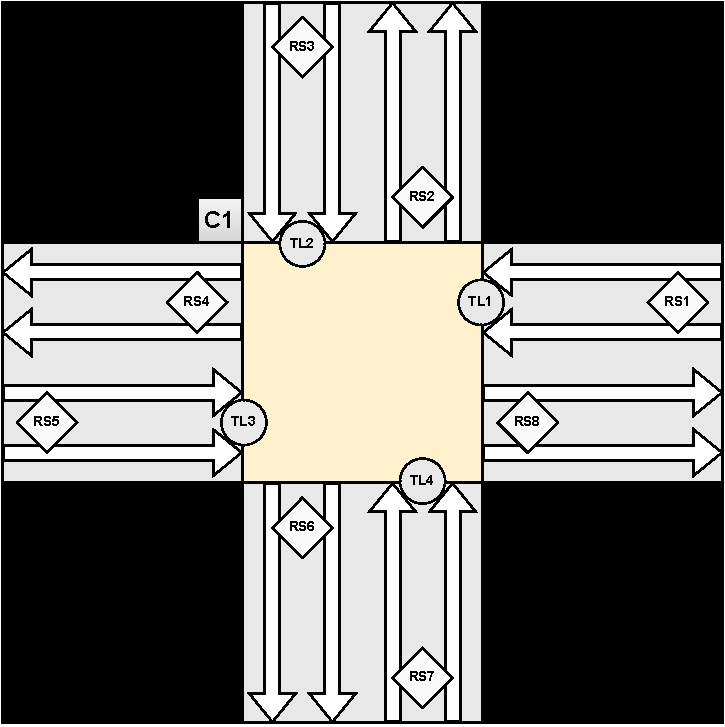
\includegraphics[width=1\linewidth]{text/image/DCruc-CEstandar-Topologia.pdf}
    \caption{Topología del cruce estándar}
    \label{fig:cruce_estandar_topologia_esc}
\end{figure}

\newpage
\section{Ciudad 6. Cruce complejo real}
    \label{section:cruce_real}
El cruce de la Avenida de la Constitución con la Avenida Doctor Olóriz y Avenida Andaluces es el escenario real que se ha representado. Es una de las intersecciones más problemáticas y con más tráfico de la ciudad de Granada.
\subsection{Marcación del cruce real}
\begin{figure}[H]
    \centering
    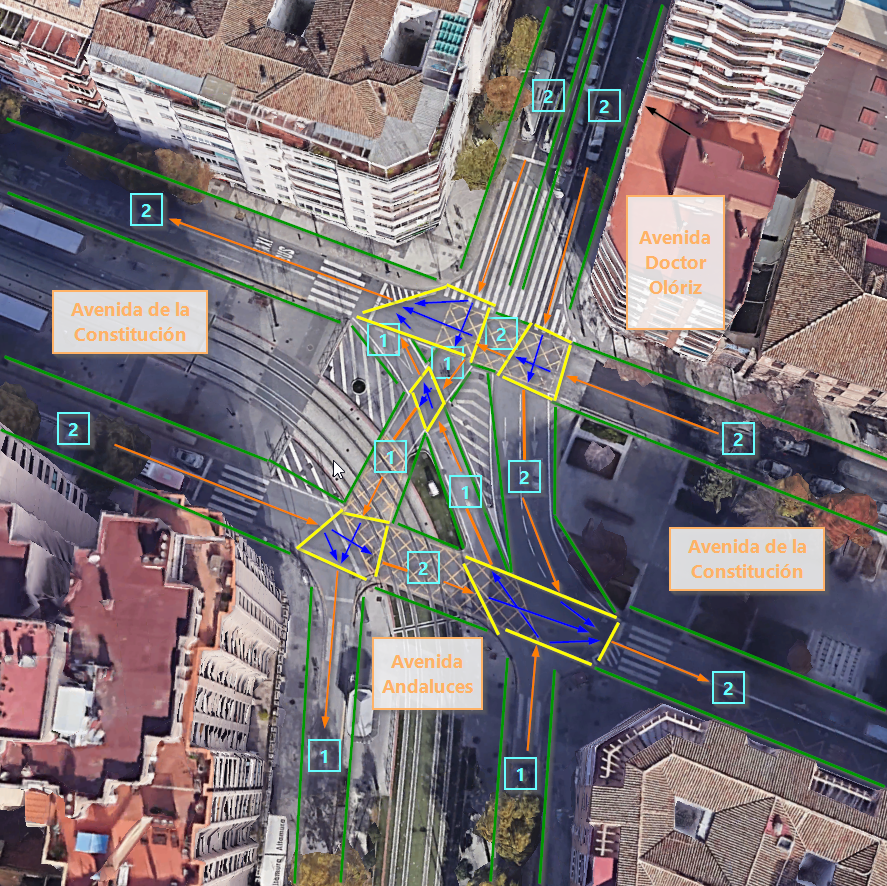
\includegraphics[width=0.95\linewidth]{text/image/DCruc-CReal.png}
    \caption{Cruce real: Avenida de la Constitución, Avenida Doctor Olóriz y Avenida Andaluces}
    \label{fig:cruce_real}
\end{figure}
Como se puede observar, el modelado del escenario consta de cinco cruces (en amarillo), quince tramos de calle (cada par de líneas verdes), doce semáforos (uno por cada tramo de calle de entrada a un cruce) y quince tramos de cruce (en azul).

\newpage
\subsection{Topología del cruce real}
Tras haber pasado el marcado del cruce real a el tipo modelo que se está utilizando, se obtendría la siguiente topología:
\begin{figure}[H]
    \centering
    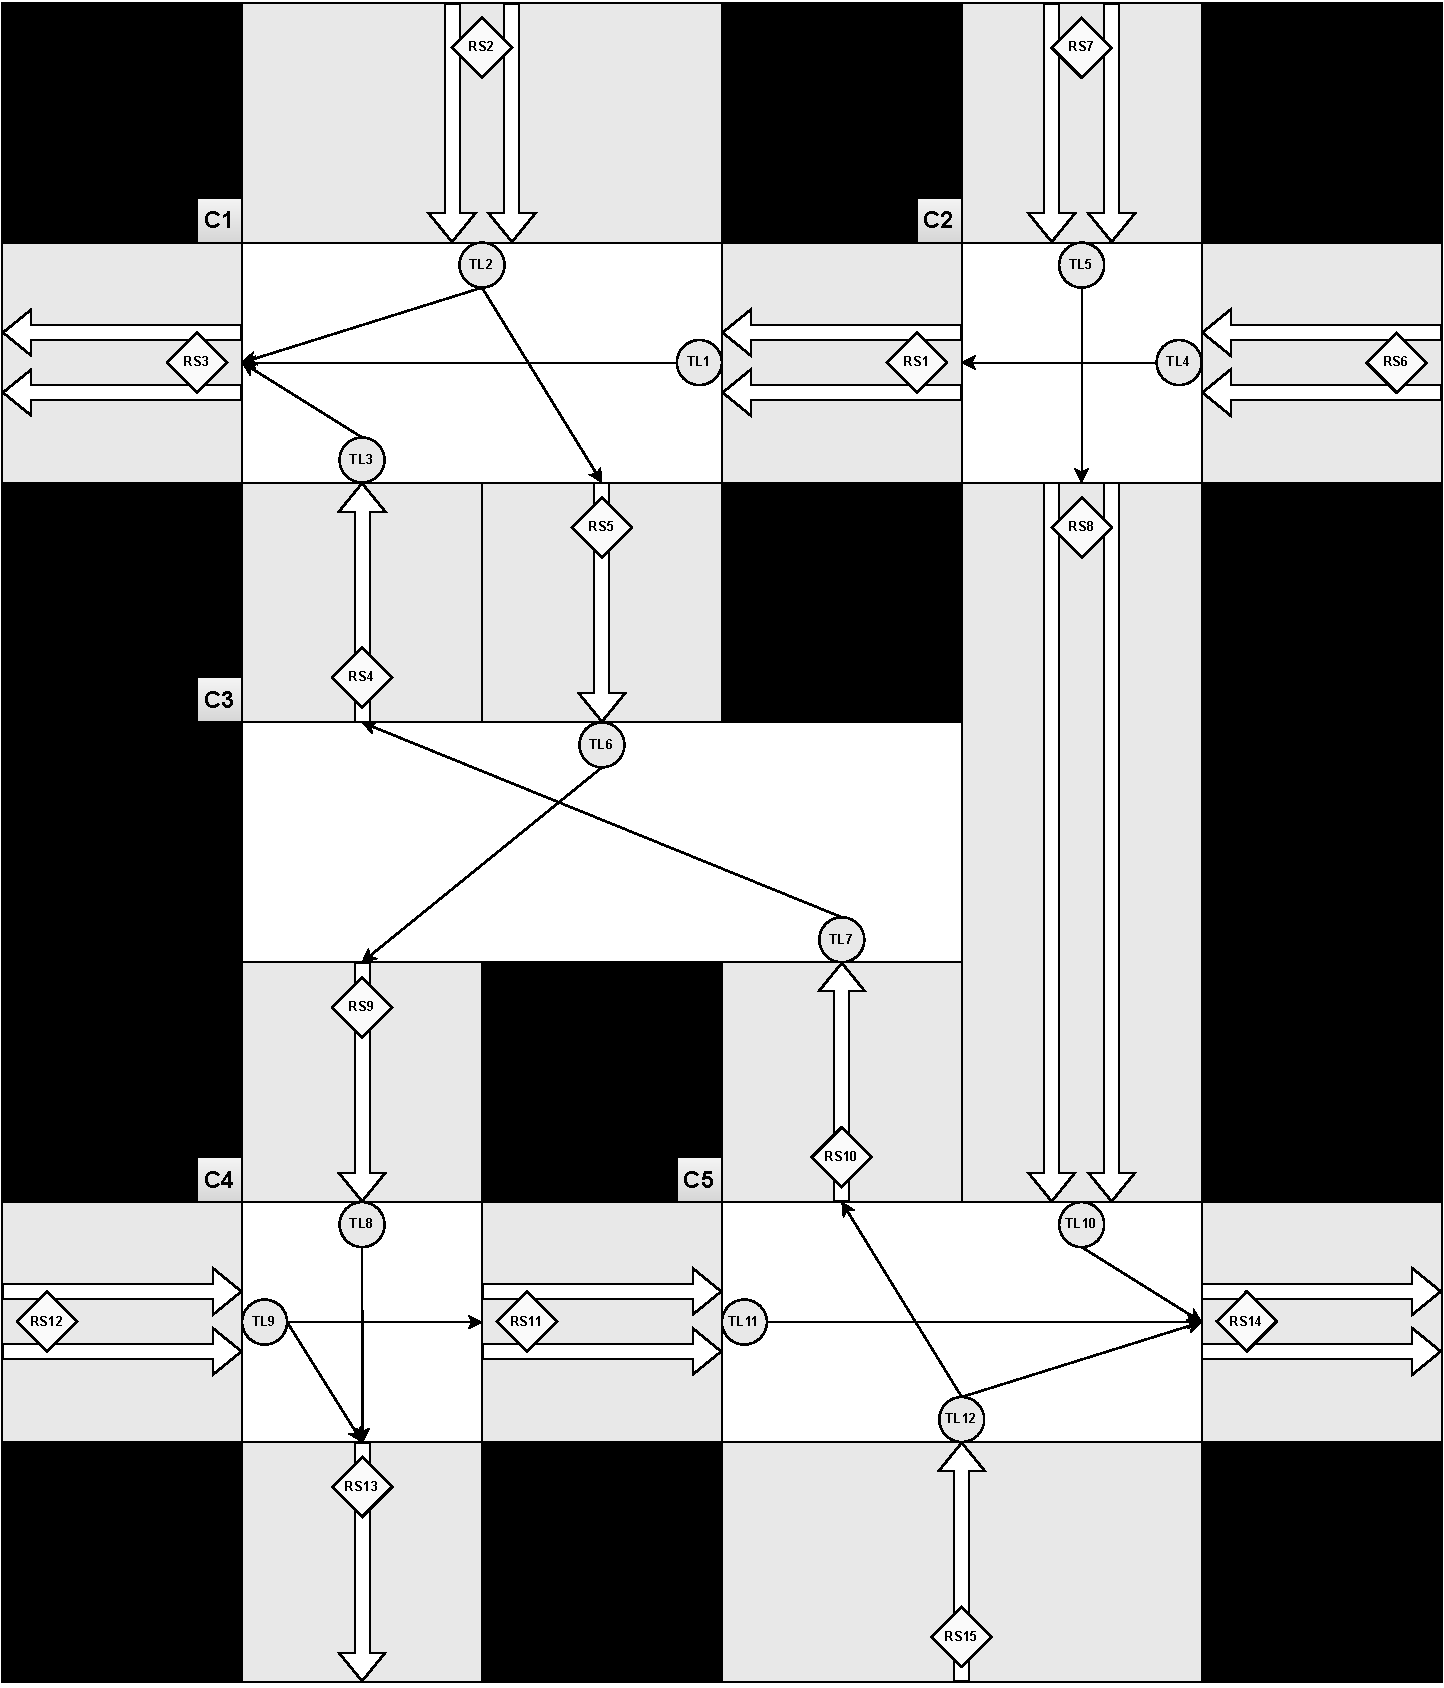
\includegraphics[width=1\linewidth]{text/image/DCruc-CReal-Topologia.pdf}
    \caption{Topología del cruce real: Avenida de la Constitución, Avenida Doctor Olóriz y Avenida Andaluces}
    \label{fig:cruce_real_topologia}
\end{figure}



\chapter{Análisis de los resultados obtenidos}
    \label{chap:seven}
    
\section{Resultados de la simulación de tráfico}
    \label{section:resultados}
    
\subsubsection{Adición de tráfico al sistema en diferentes modos}
    \label{subsubsection:adicion_trafico}
Los ejemplos de adición de vehículos se han realizado en base al escenario representado en la figura \ref{fig:cruce_estandar_topologia_esc} con tres configuraciones idénticas con la única variación del modo de adición de vehículos.


Para el modo lineal de adición de tráfico, tal y como se puede observar en la figura \ref{fig:adicion_trafico_lineal}, entra al sistema de tráfico la misma cantidad de vehículos durante toda la simulación.
\begin{figure}[H]
    \centering
    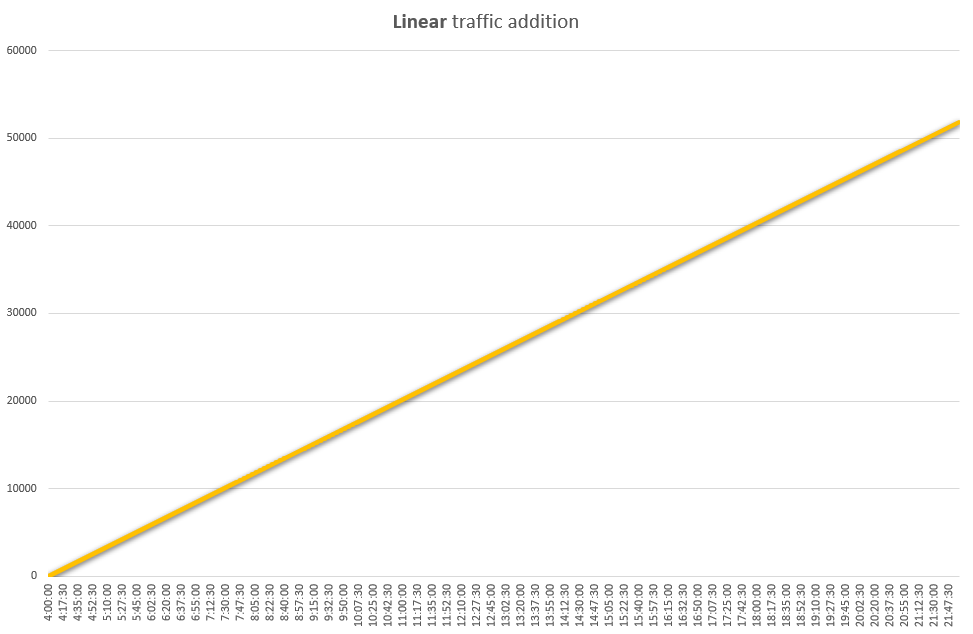
\includegraphics[width=0.81\linewidth]{text/image/Linear.png}
    \caption{Adición de tráfico al sistema en modo lineal (\textit{LINEAR})}
    \label{fig:adicion_trafico_lineal}
\end{figure}

Para el modo de pico único de adición de tráfico, como se puede apreciar en la figura \ref{fig:adicion_trafico_single_peak}, durante toda la simulación entra al sistema de tráfico la misma cantidad de vehículos a excepción de en un intervalo pico determinado, donde entra una cantidad
mucho mayor. Este pico de tráfico sucede entre las ocho y las nueve de la mañana.
\begin{figure}[H]
    \centering
    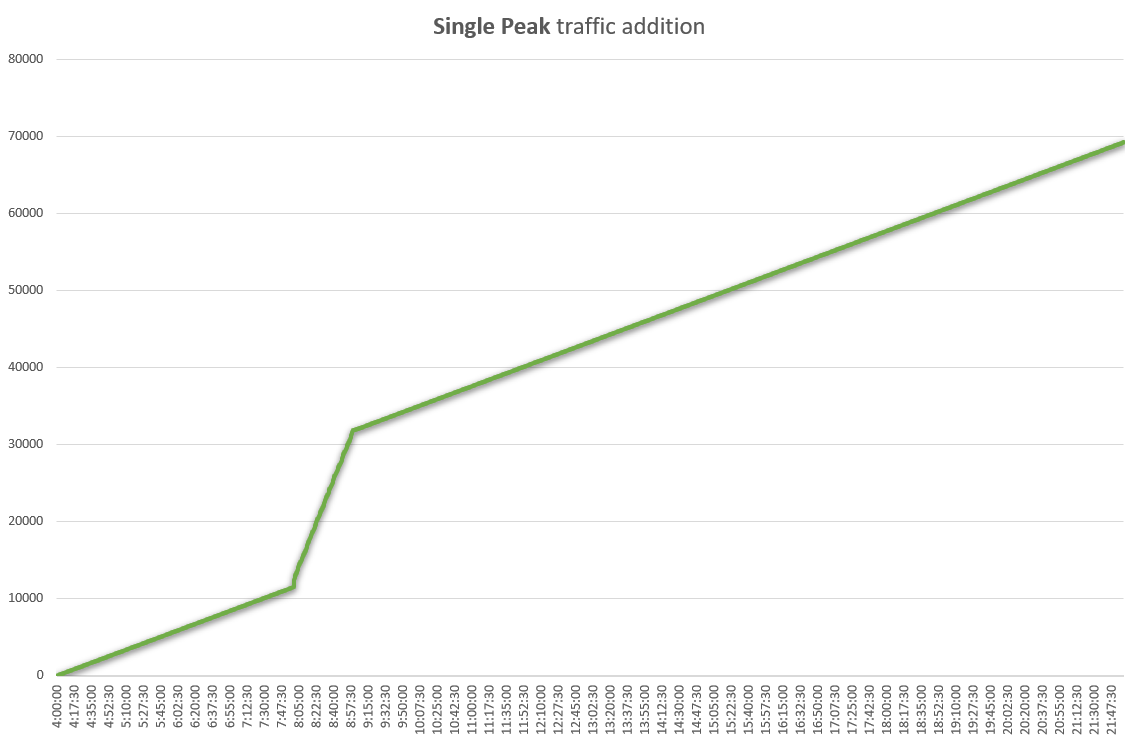
\includegraphics[width=1\linewidth]{text/image/SinglePeak.png}
    \caption{Adición de tráfico al sistema en modo pico único (\textit{SINGLE\_PEAK})}
    \label{fig:adicion_trafico_single_peak}
\end{figure}

\newpage
Para el modo de doble pico de adición de tráfico, tal y como se puede percibir en la figura \ref{fig:adicion_trafico_double_peak}, durante toda la simulación es añadida al sistema de tráfico la misma cantidad de vehículos a excepción de en un intervalo pico determinado, donde entra una cantidad mucho mayor. Estos picos de tráfico suceden entre: las ocho y las nueve de la mañana; y las dos y las tres de la tarde.
\begin{figure}[H]
    \centering
    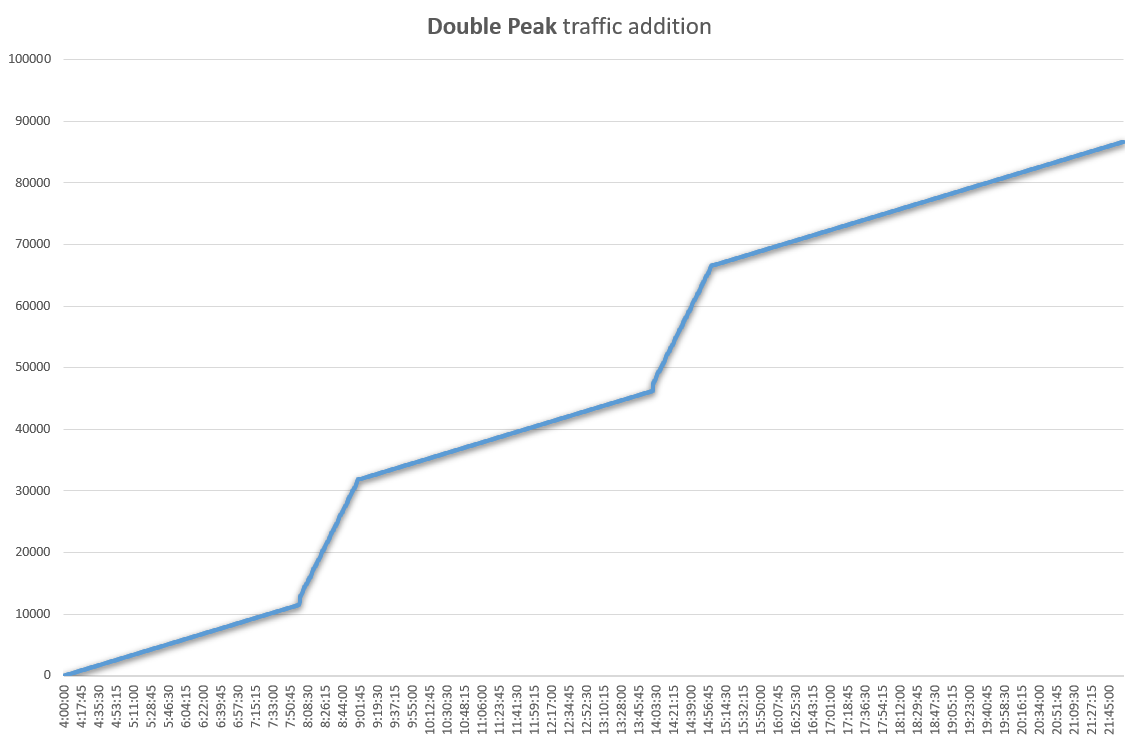
\includegraphics[width=1\linewidth]{text/image/DoublePeak.png}
    \caption{Adición de tráfico al sistema en modo doble pico (\textit{DOUBLE\_PEAK})}
    \label{fig:adicion_trafico_double_peak}
\end{figure}

\newpage
Comparando los tres modos de adición de vehículos, se puede observar que cuantos más intervalos pico existan en la simulación mayor cantidad de vehículos es añadida durante el transcurso de la misma.
\begin{figure}[H]
    \centering
    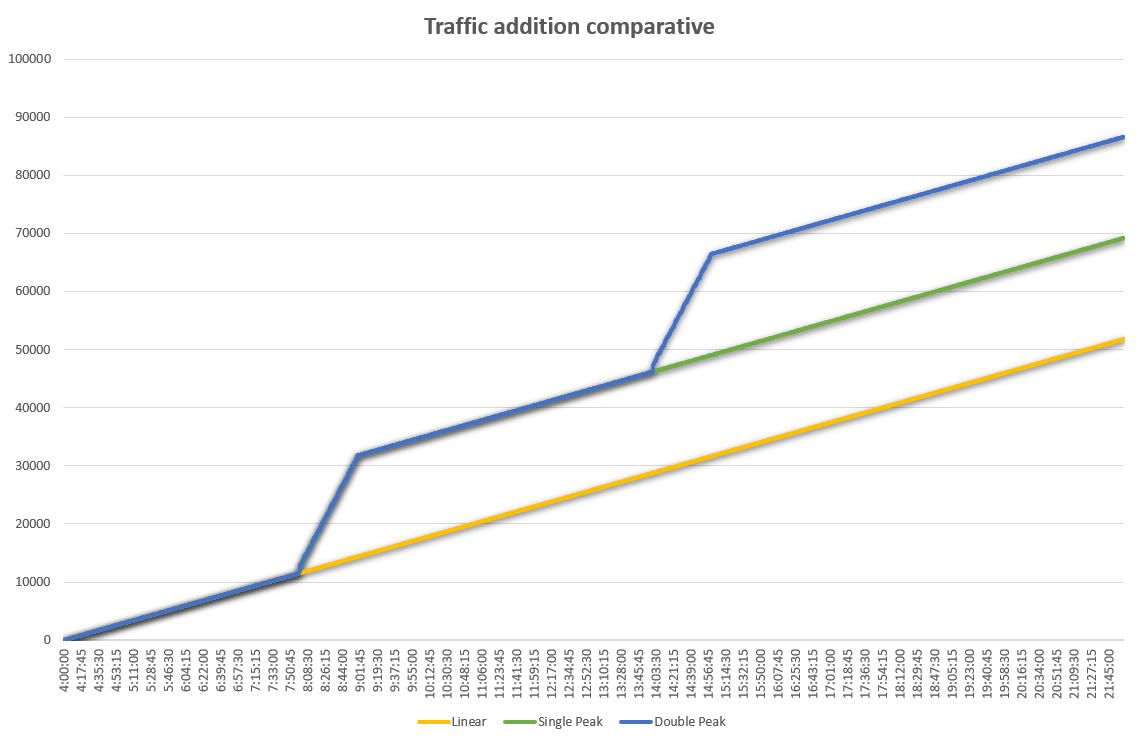
\includegraphics[width=1\linewidth]{text/image/TrafficAdition.png}
    \caption{Comparativa de adición de tráfico al sistema en los tres modos disponibles}
    \label{fig:adicion_trafico_comparativa}
\end{figure}

Para la simulación con modo de entrada de tráfico \textbf{lineal} se han añadido al sistema de tráfico la cantidad de \textbf{51840} vehículos. Es el modo en el que menos vehículos se han añadido.

Para la simulación con modo de entrada de tráfico de \textbf{pico único} se han añadido al sistema de tráfico la cantidad de \textbf{69263} vehículos. Un \textbf{33,61\%} más que en el modo \textbf{lineal}.

Para la simulación con modo de entrada de tráfico de \textbf{doble pico} se han añadido al sistema de tráfico la cantidad de \textbf{86686} vehículos. Un \textbf{67,22\%} más que en el modo \textbf{lineal} y un \textbf{25,15\%} más que en el modo de \textbf{pico único}. Es el modo en el que más vehículos se han añadido.

Como conclusión, se puede afirmar que existe la posibilidad de añadir grandes cantidades de vehículos al sistema en intervalos determinados, lo cual es muy útil para generar situaciones de congestión.

\newpage
\subsubsection{Tráfico procesado por la simulación}
Las gráficas que se muestran en esta sección han sido obtenidas a partir de dos simulaciones realizadas, una con política de tiempos fijos y otra con política de tiempos variables, en base al escenario representado en la figura \ref{fig:cruce_simple2x1_topologia}.

Como se puede observar en la figura \ref{fig:vehicles_in_city2}, la adición de tráfico al sistema se ha realizado en modo doble pico. Dicha gráfica muestra el valor acumulado de vehículos que han entrado al sistema durante cada una de las simulaciones.
\begin{figure}[H]
    \centering
    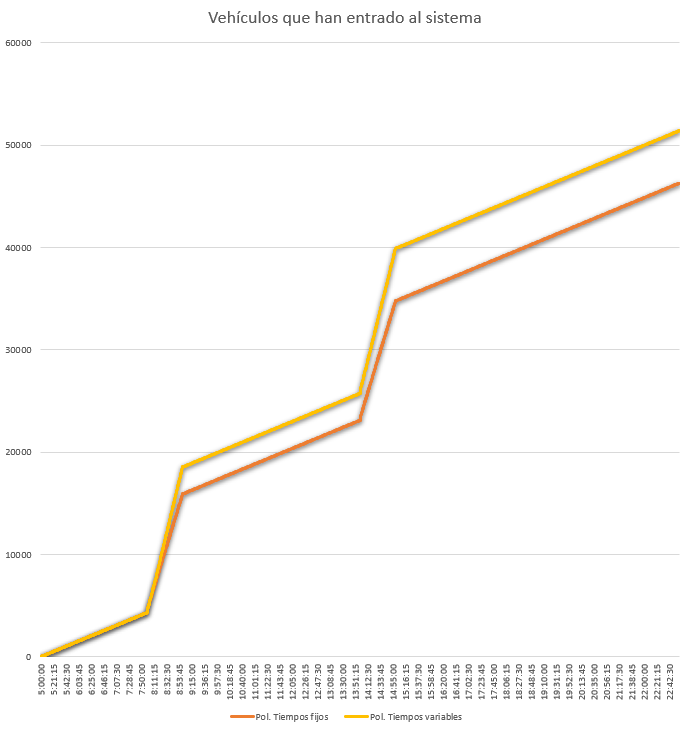
\includegraphics[width=0.80\linewidth]{text/image/SIMvehiclesInCITY2-CONFIG2.png}
    \caption{Vehículos acumulados que han entrado al sistema}
    \label{fig:vehicles_in_city2}
\end{figure}
\begin{itemize}
    \item Con la política de \textbf{tiempos fijos} han entrado al sistema \textbf{46284} vehículos.
    \item Con la política de \textbf{tiempos variables} han entrado al sistema \textbf{51403} vehículos.
\end{itemize}
Aplicando una política de tiempos variables, el sistema de tráfico ha sido capaz de absorber alrededor de un \textbf{11,06\%} más de vehículos.


Como se puede observar en la figura \ref{fig:vehicles_out_city2}, la gráfica de vehículos que salen del sistema es prácticamente igual a la de los vehículos que entran. Dicha gráfica muestra el valor acumulado de vehículos que han sido procesados por el sistema durante cada una de las simulaciones. Los valores obtenidos evidencian que la mayoría de los vehículos que entran, salen del sistema.
\begin{figure}[H]
    \centering
    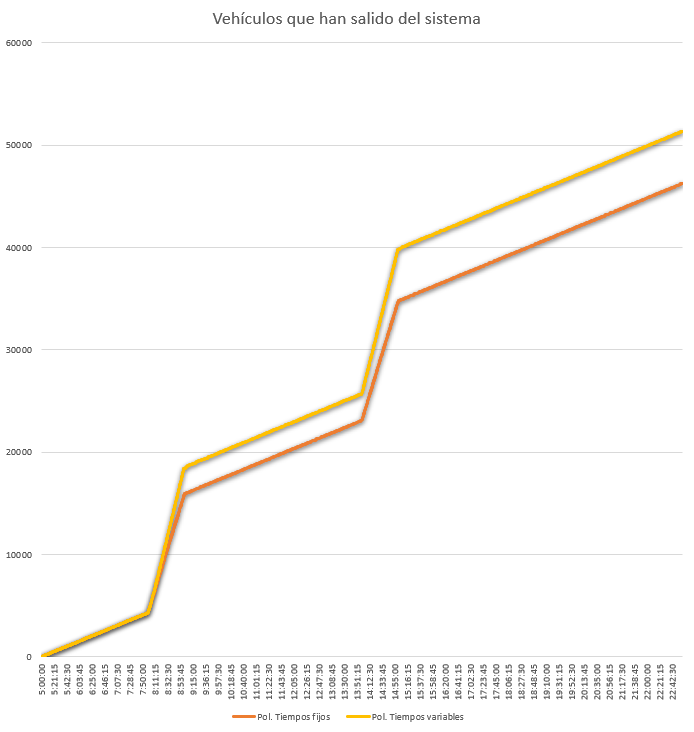
\includegraphics[width=0.80\linewidth]{text/image/SIMvehiclesOutCITY2-CONFIG2.png}
    \caption{Vehículos acumulados que han salido del sistema}
    \label{fig:vehicles_out_city2}
\end{figure}
\begin{itemize}
    \item Con la política de \textbf{tiempos fijos} el sistema ha procesado \textbf{46248} vehículos.
    \item Con la política de \textbf{tiempos variables} el sistema ha procesado \textbf{51357} vehículos.
\end{itemize}
Aplicando una política de tiempos variables, el sistema de tráfico ha sido capaz de procesar alrededor de un \textbf{11,05\%} más de vehículos.

Al final de la simulación quedan en el sistema: aplicando la política de tiempos fijos, 36 vehículos (0,077\% del total) que han entrado pero a los que no les ha dado tiempo a salir; aplicando la política de tiempos variables, 46 vehículos (0,089\% del total) que han entrado pero a los que no les ha dado tiempo a salir.

Analizando las figuras \ref{fig:vehicles_in_city2} y \ref{fig:vehicles_out_city2} se puede apreciar que las mejoras empiezan a producirse a partir del primer intervalo pico, lo cual es lógico, debido a que es el primer intervalo en el que se empiezan a producir condiciones de congestión en los cruces. Cuando no hay condiciones de congestión la entrada y salida de vehículos al sistema es similar, esto es debido a que se pueden absorber y procesar vehículos de forma normal. En el segundo intervalo pico se puede ver que sucede algo similar a lo que sucede en el primero, se producen situaciones de congestión, ergo se optimizan los tiempos y se pueden absorber y generar más vehículos.

La figura \ref{fig:vehicles_total_city2} muestra los vehículos totales en el sistema en cada instante de cada una de las simulaciones. Al igual que sucedía en los gráficos ya explicados, los valores de vehículos totales de la simulación con política de tiempos fijos (color naranja) son similares a los de la simulación con política de tiempos variables (color amarillo) hasta el inicio de la primera hora pico. Esto sucede porque hasta dicho momento no se aplica la optimización de tiempos de estados. En el momento en el se aplica la optimización de tiempos se puede apreciar que el número de vehículos totales aumenta en la simulación cuya política es de tiempos variables con respecto a la simulación cuya política es de tiempos fijos. Se puede ver claramente como durante el resto de la simulación, tras haber habido situaciones de congestión, hay más vehículos en la simulación con la política de tiempos variables. 

\begin{figure}[H]
    \centering
    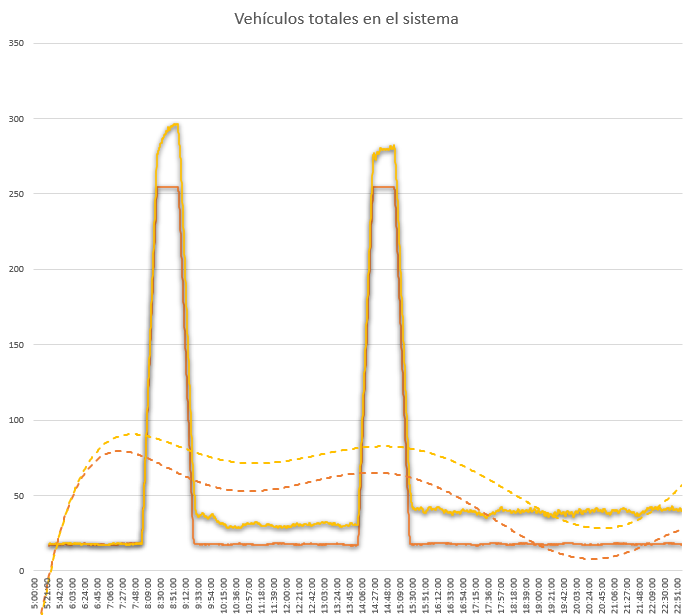
\includegraphics[width=0.84\linewidth]{text/image/SIMtotalVehiclesCITY2-CONFIG2.png}
    \caption{Vehículos totales en cada instante de las simulaciones}
    \label{fig:vehicles_total_city2}
\end{figure}

En el gráfico de la figura \ref{fig:ticks_exit_city2} se puede ver el tiempo medio acumulado que tardan los vehículos en salir de la simulación. Como se puede observar, justo al inicio de la gráfica hay un aumento considerable de tiempo medio, que hace que se sitúe en un valor de alrededor de 60 segundos. Al inicio de la simulación no hay ningún vehículo en el sistema. Los vehículos empiezan a ser añadidos poco a poco en todos los tramos de calle de entrada al sistema. Esto produce que algunos vehículos salgan de forma casi inmediata porque el estado inicial del cruce les beneficie y otros vehículos tengan que esperar detrás de un semáforo en rojo. Lo anterior produce que el valor medio de tiempo que tarda un vehículo en salir se sitúe alrededor del ya mencionado.
\begin{figure}[H]
    \centering
    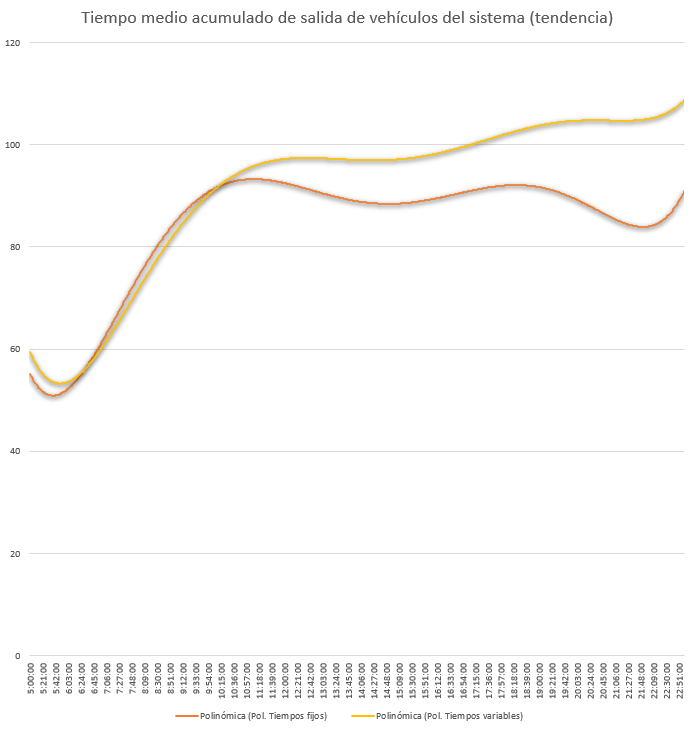
\includegraphics[width=0.84\linewidth]{text/image/SIMaverageTicksToExitTendenciaCITY2-CONFIG2.png}
    \caption{Tiempo medio acumulado que tarda un vehículo en salir del sistema}
    \label{fig:ticks_exit_city2}
\end{figure}
A partir de la estabilización inicial, el valor se mantiene más o menos constante hasta que llega el primer intervalo pico. Al añadirse tantos vehículos al sistema, el tiempo que tarda de media un vehículo desde que entra hasta que sale del mismo aumenta. La razón es sencilla, esto es debido a que la cola de vehículos para entrar a los cruces es más larga y, por lo tanto, el tiempo de espera es mayor. Una vez finaliza el la hora pico, el tiempo medio disminuye poco a poco conforme se va desalojando el sistema. Evidentemente, en la simulación cuya política es de tiempos variables, al procesar un mayor número de vehículos, las colas son más largas y el tiempo medio que tarda un vehículo en salir del sistema es mayor.

\newpage
\section{Resultados de seguimiento del proyecto}
Un burndown chart es una gráfica en la que se puede ver el estado del progreso de un proyecto en un sprint, en una release, en el proyecto completo o en aquel período que se haya establecido.

Para construir este gráfico es necesaria determinada información:
\begin{itemize}
    \item \textbf{Tiempo}. Corresponde al eje X de la gráfica. Representa para $x=0$ el inicio del periodo temporal y para $x=t$ el final del periodo temporal. Estos dos valores se corresponden, por ejemplo, en el burndown chart global del proyecto con las fechas de inicio y finalización del mismo.
    \item \textbf{Cantidad de trabajo}. Corresponde al eje Y de la gráfica. Representa el trabajo planificado que se debe realizar durante el tiempo medido. Cuando se estiman las tareas, independientemente de la unidad de estimación que se utilice, se obtiene un valor que indica la cantidad de trabajo a realizar. El valor de cantidad de trabajo restante debe ir decreciendo en relación al tiempo que va avanzando.
    \item \textbf{Referencia ideal}. Corresponde a la línea que diagonal trazada desde la parte superior izquierda hasta la parte inferior derecha. Representa la relación ideal entre la disminución de la cantidad de trabajo y el tiempo que se debería producirse durante el transcurso de la fase correspondiente. Cuanto más se aproxime la línea real a la linea ideal se podría decir que se está trabajando de mejor forma en relación a la consecución de objetivos.
\end{itemize}

Además de lo anterior, si se tiene el conocimiento y la experiencia suficiente trabajando con estas herramientas ágiles, se puede obtener mucha información útil sobre el seguimiento del proyecto. Esta información puede servir, entre otras muchas cosas, para impulsar las buenas prácticas y promover el mismo desarrollo del proyecto. 

\subsection{Burndown chart global del proyecto}
Observando el burndown chart global del proyecto, expuesto en la figura \ref{fig:burndown_chart_proyecto}, se pueden apreciar varias cosas interesantes:
\begin{itemize}
    \item Hay un tramo de la curva totalmente plano. Como posteriormente se explicará, este tramo corresponde a un período en el que no se ha realizado trabajo.
    \item Prácticamente hasta final del proyecto, se ha ido siempre por detrás del trabajo estimado. Sin embargo, esto se debe a algunos periodos en los que se ha trabajado menos, como el mencionado arriba. 
    \item En muchos periodos, como se puede ver, se ha realizado más trabajo del planificado, son los períodos en los que la línea roja se aproxima más a la línea azul.
    \item Desde la mitad del proyecto en adelante, aproximadamente, se ha realizado más trabajo del planificado. Esto ha conseguido compensar la diferencia que se había producido anteriormente.
\end{itemize}
Se puede concluir con que, de forma global, se ha realizado la cantidad de trabajo planificada antes de lo previsto. Además, pese a la diferencia existente en algunos puntos con para la situación ideal, se ha logrado mantener bajo control el proyecto durante los diferentes sprints. Gracias a este seguimiento se han podido valorar en cada momento los riesgos existentes y se han tomando acciones en relación a estos, por ejemplo, en forma de compensación de trabajo siempre que ha sido necesario debido a las horas no realizadas en periodos anteriores.

\begin{figure}[H]
    \centering
    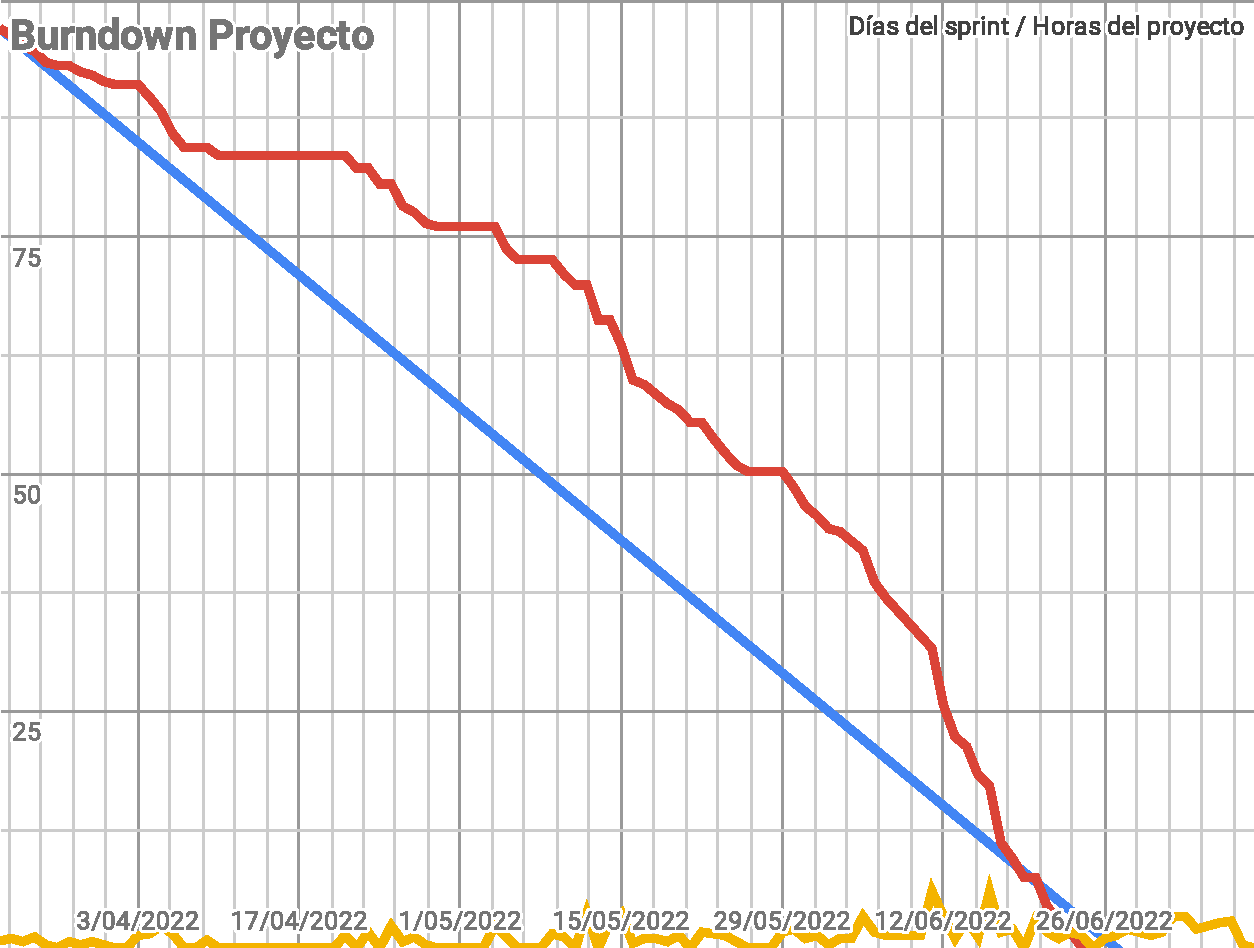
\includegraphics[width=1\linewidth]{text/image/BurndownChartGlobal.pdf}
    \caption{Burndown chart $|$ Proyecto $|$ del 22/03 al 08/07}
    \label{fig:burndown_chart_proyecto}
\end{figure}

\newpage
\subsection{Burndown charts de cada sprint}
Durante el transcurso de cada sprint, se ha realizado el seguimiento tanto particular de dicho sprint como global de todo el proyecto. Gracias a esto, se ha podido tener una perspectiva global de la evolución del mismo.

\paragraph{Sprint 1 (del 22/03 al 05/04)} 
Durante los primeros días del sprint se mantuvo un trabajo constante en relación a lo que estaba previsto. Tras esto, la cantidad de trabajo realizada se redujo y, aun trabajando diariamente, la cantidad de trabajo realizada no era suficiente. Al final del sprint aumentó de nuevo el trabajo diario realizado, sin embargo, no se pudo completar toda la cantidad de trabajo prevista para el sprint.
\begin{figure}[H]
    \centering
    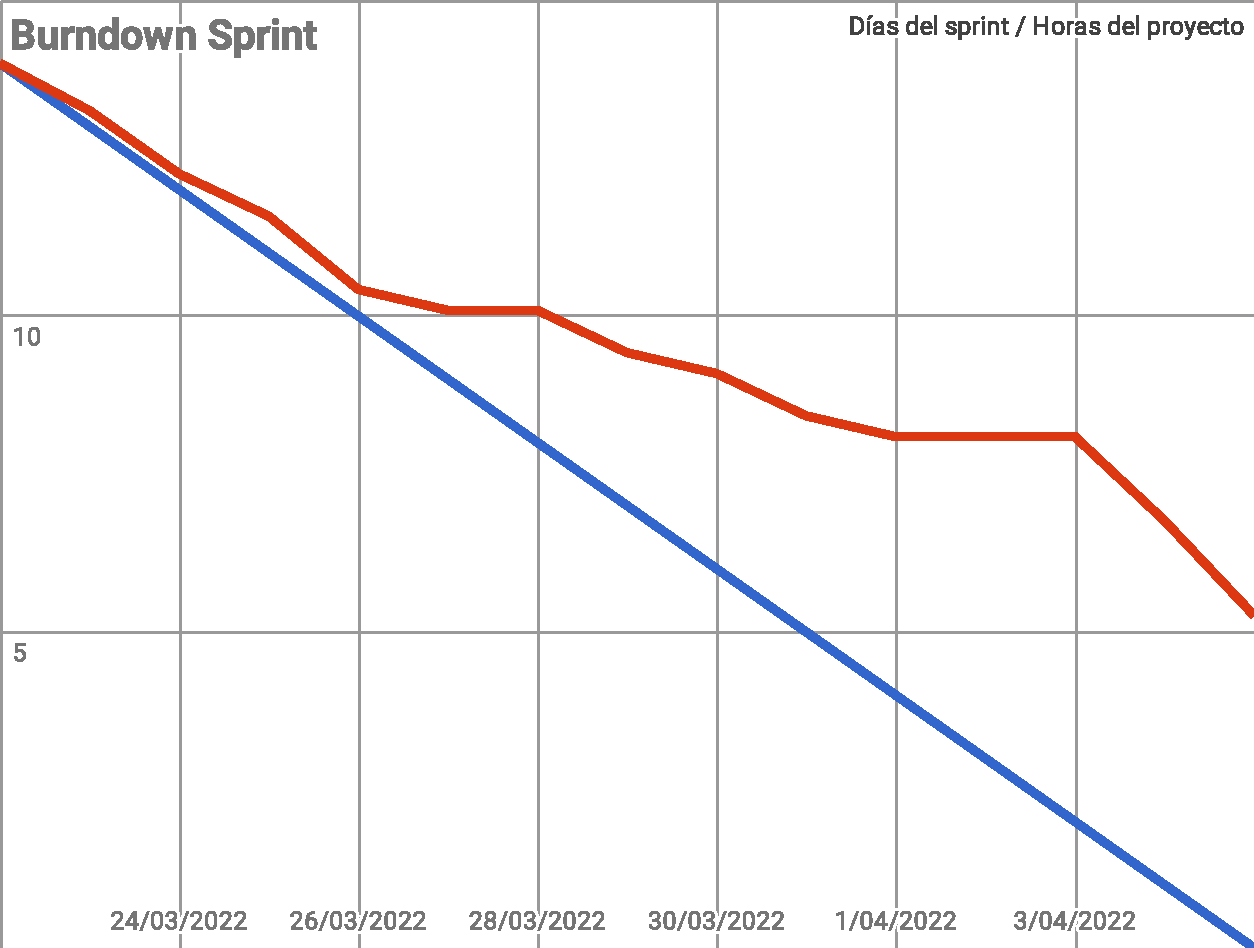
\includegraphics[width=1\linewidth]{text/image/BurndownChart1.pdf}
    \caption{Burndown chart $|$ Sprint 1 $|$ del 22/03 al 05/04}
    \label{fig:burndown_chart_1}
\end{figure}

\newpage
\paragraph{Sprint 2 (del 06/04 al 20/04)}
Este sprint es algo totalmente anormal, que no se debe dar. La razón es simple, si la línea roja permanece horizontal es porque no se está trabajando. No obstante, es correcto porque inicialmente se planificó que durante el periodo vacacional de Semana Santa no se iba a trabajar. Habría sido interesante omitir este periodo del seguimiento, sin embargo, se ha considerado interesante para mostrar una tendencia mala en relación al desarrollo del proyecto.
\begin{figure}[H]
    \centering
    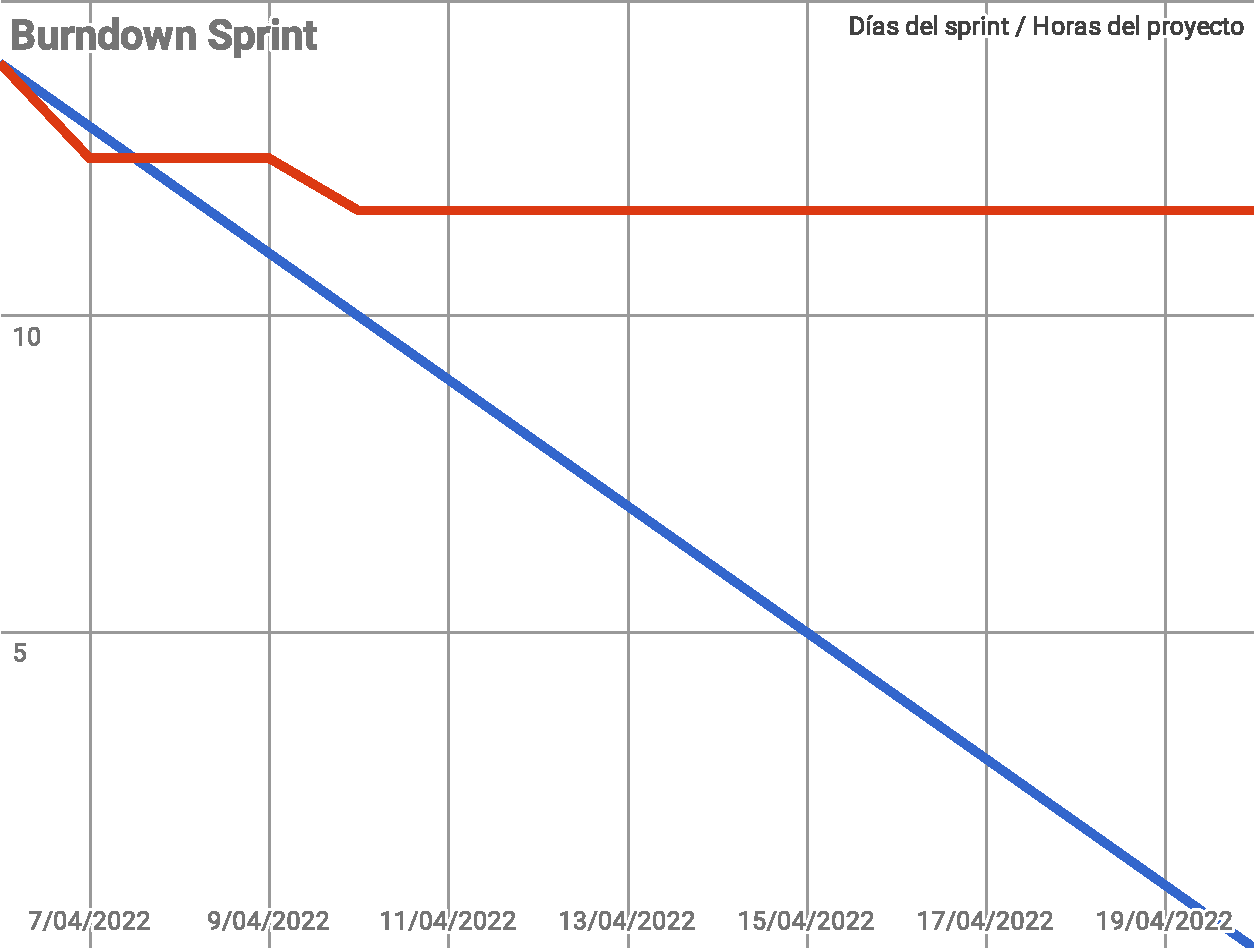
\includegraphics[width=1\linewidth]{text/image/BurndownChart2.pdf}
    \caption{Burndown chart $|$ Sprint 2 $|$ del 06/04 al 20/04}
    \label{fig:burndown_chart_2}
\end{figure}

\newpage
\paragraph{Sprint 3 (del 21/04 al 05/05)}
Se puede apreciar que la tendencia es muy buena durante la primera parte del sprint. Hasta la mitad del periodo la curva roja se sitúa alrededor de la tendencia ideal, lo cual manifiesta que el sprint está controlado. Posteriormente, se puede observar un parón hasta el día previo a la finalización del sprint, donde se realizó una cantidad de trabajo considerable.
\begin{figure}[H]
    \centering
    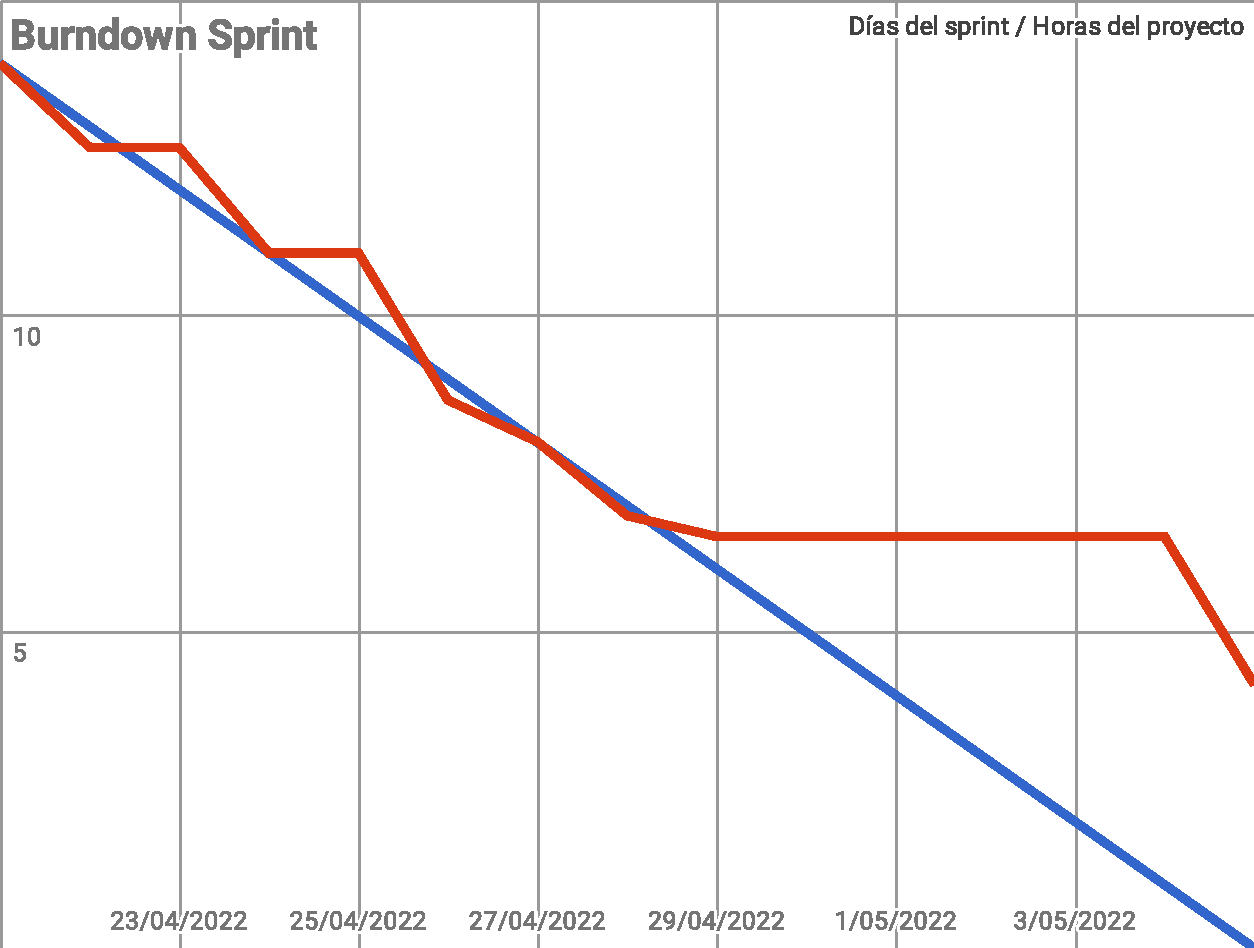
\includegraphics[width=1\linewidth]{text/image/BurndownChart3.pdf}
    \caption{Burndown chart $|$ Sprint 3 $|$ del 21/04 al 05/05}
    \label{fig:burndown_chart_3}
\end{figure}

\newpage
\paragraph{Sprint 4 (del 06/05 al 20/05)}
El gráfico de este sprint muestra que se realizaron grandes cantidades de trabajo en días concretos. Se puede apreciar que algo después de pasar la mitad del tiempo del sprint, se consiguió cortar la curva ideal con la curva de trabajo real, realizando en los días anteriores y posteriores mucha más cantidad de trabajo de la que estaba planificada. Esto, en cierto modo, sirvió para compensar parte del trabajo no realizado en sprints anteriores.
\begin{figure}[H]
    \centering
    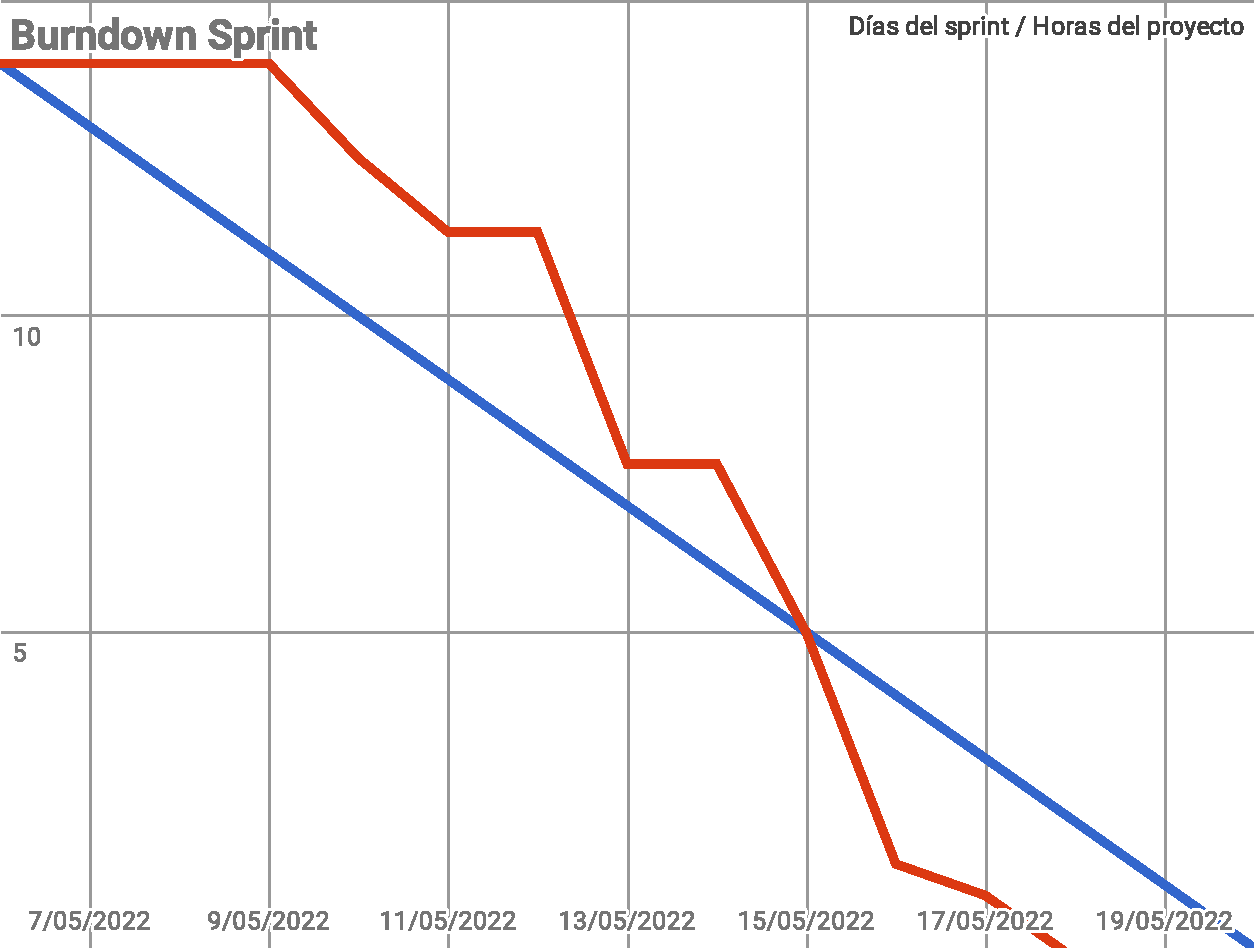
\includegraphics[width=1\linewidth]{text/image/BurndownChart4.pdf}
    \caption{Burndown chart $|$ Sprint 4 $|$ del 06/05 al 20/05}
    \label{fig:burndown_chart_4}
\end{figure}

\newpage
\paragraph{Sprint 5 (del 21/05 al 04/06)}
Durante el presente sprint, se mantuvo una tendencia adecuada hasta, aproximadamente, un poco antes de la mitad del mismo. A partir de ese momento hubo un par de días de parón, los cuales, posteriormente, se compensaron en casi su totalidad.
\begin{figure}[H]
    \centering
    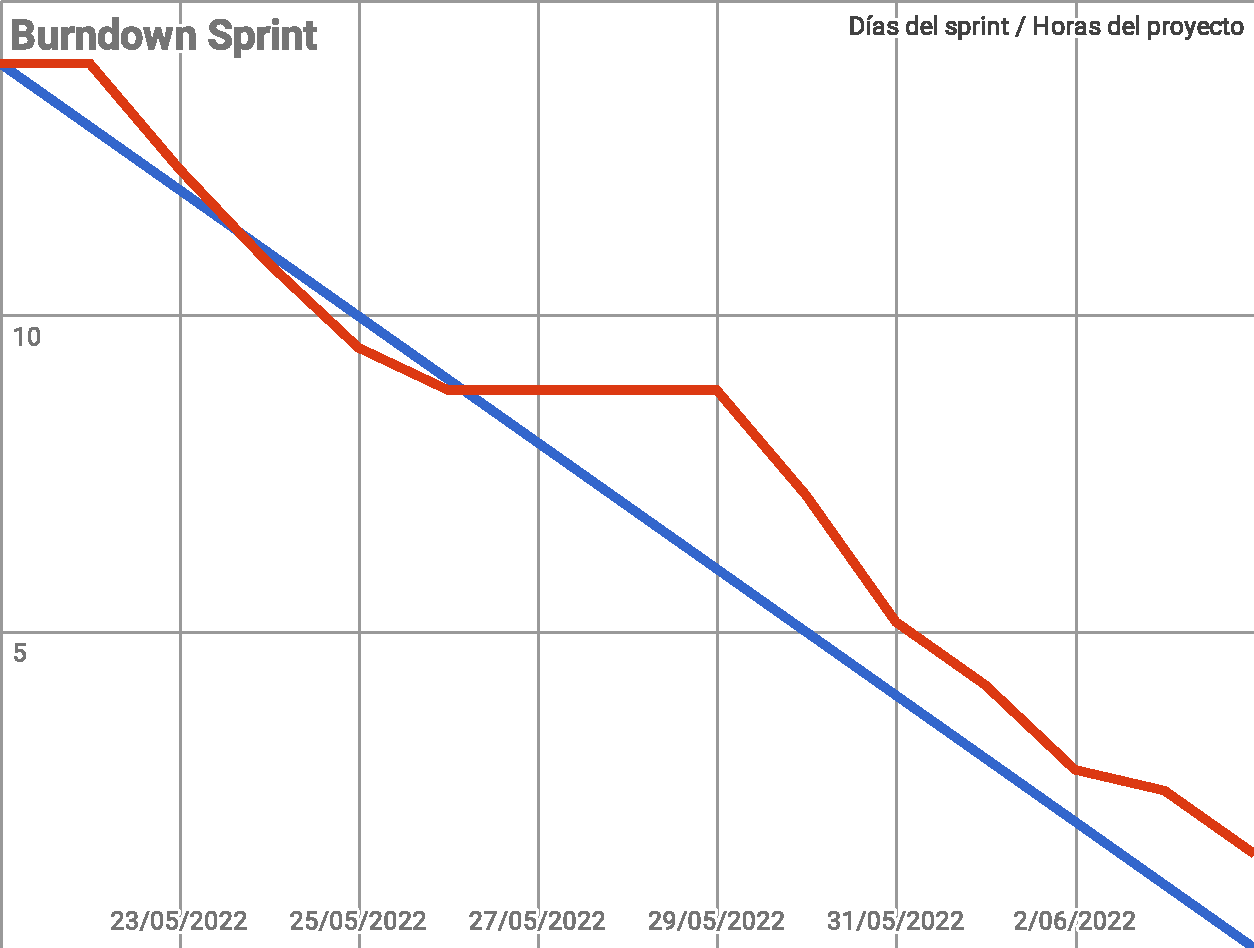
\includegraphics[width=1\linewidth]{text/image/BurndownChart5.pdf}
    \caption{Burndown chart $|$ Sprint 5 $|$ del 21/05 al 04/06}
    \label{fig:burndown_chart_5}
\end{figure}

\newpage
\paragraph{Sprint 6 (del 05/06 al 19/06)}
Claramente, se puede ver que en este sprint se realizó una cantidad de trabajo mucho más alta de lo que estaba planificado. Sin embargo, si se analiza desde un punto de vista global, se puede entender que al acercarse el final de proyecto es necesario invertir más tiempo y compensar la cantidad de trabajo que en sprints anteriores no se llegó a completar.
\begin{figure}[H]
    \centering
    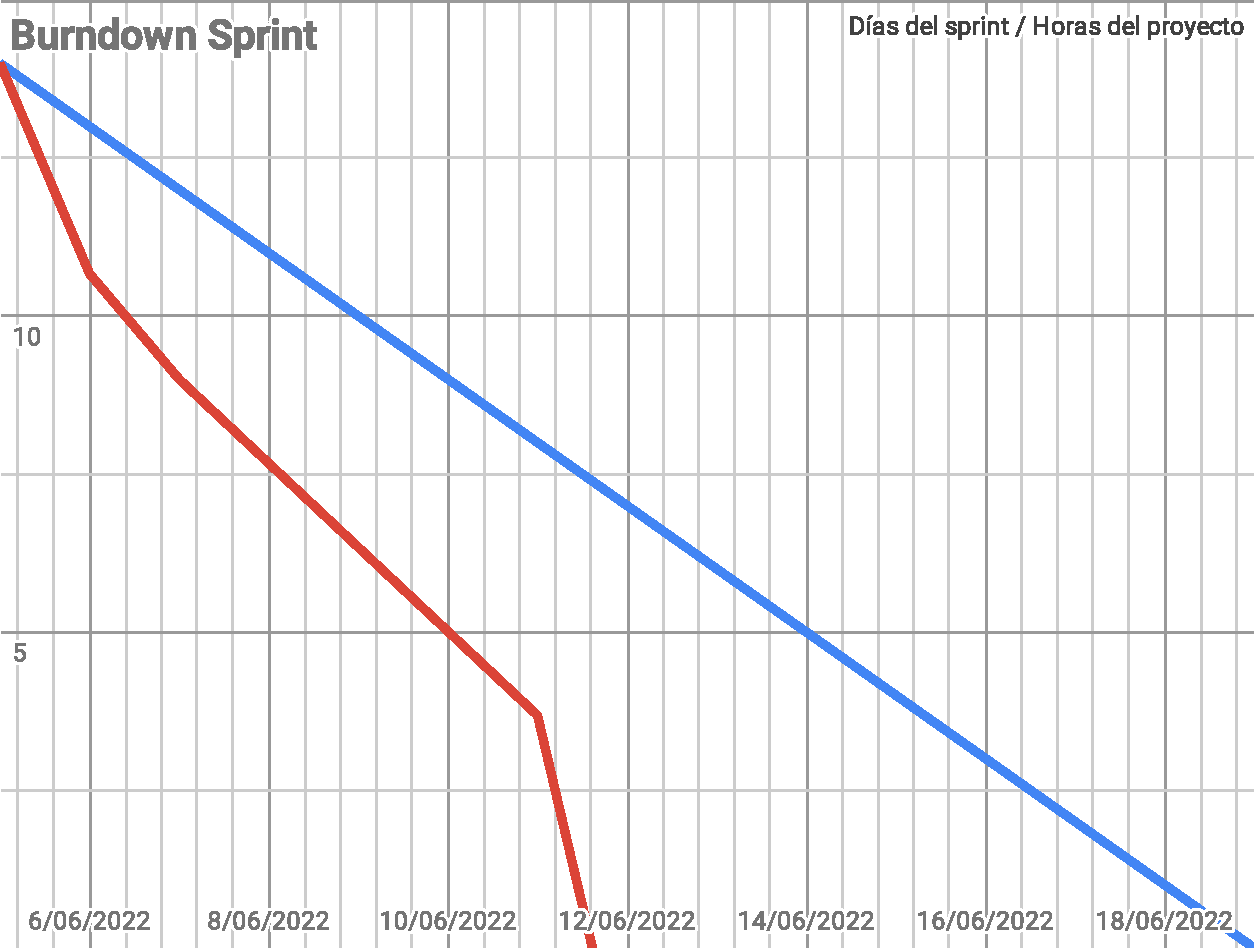
\includegraphics[width=1\linewidth]{text/image/BurndownChart6.pdf}
    \caption{Burndown chart $|$ Sprint 6 $|$ del 05/06 al 19/06}
    \label{fig:burndown_chart_6}
\end{figure}

\newpage
\paragraph{Sprint 7 (del 20/06 al 04/07)}
De manera similar al sprint anterior, se puede ver que en este sprint se realizó una cantidad de trabajo mucho más alta de lo que estaba planificado. Si que comparan ambos diagramas se puede apreciar que la tendencia es muy parecida. Esto se debe a que al ser parte de la fase final del proyecto se realizaron todas las horas de trabajo necesarias para finalizarlo.
\begin{figure}[H]
    \centering
    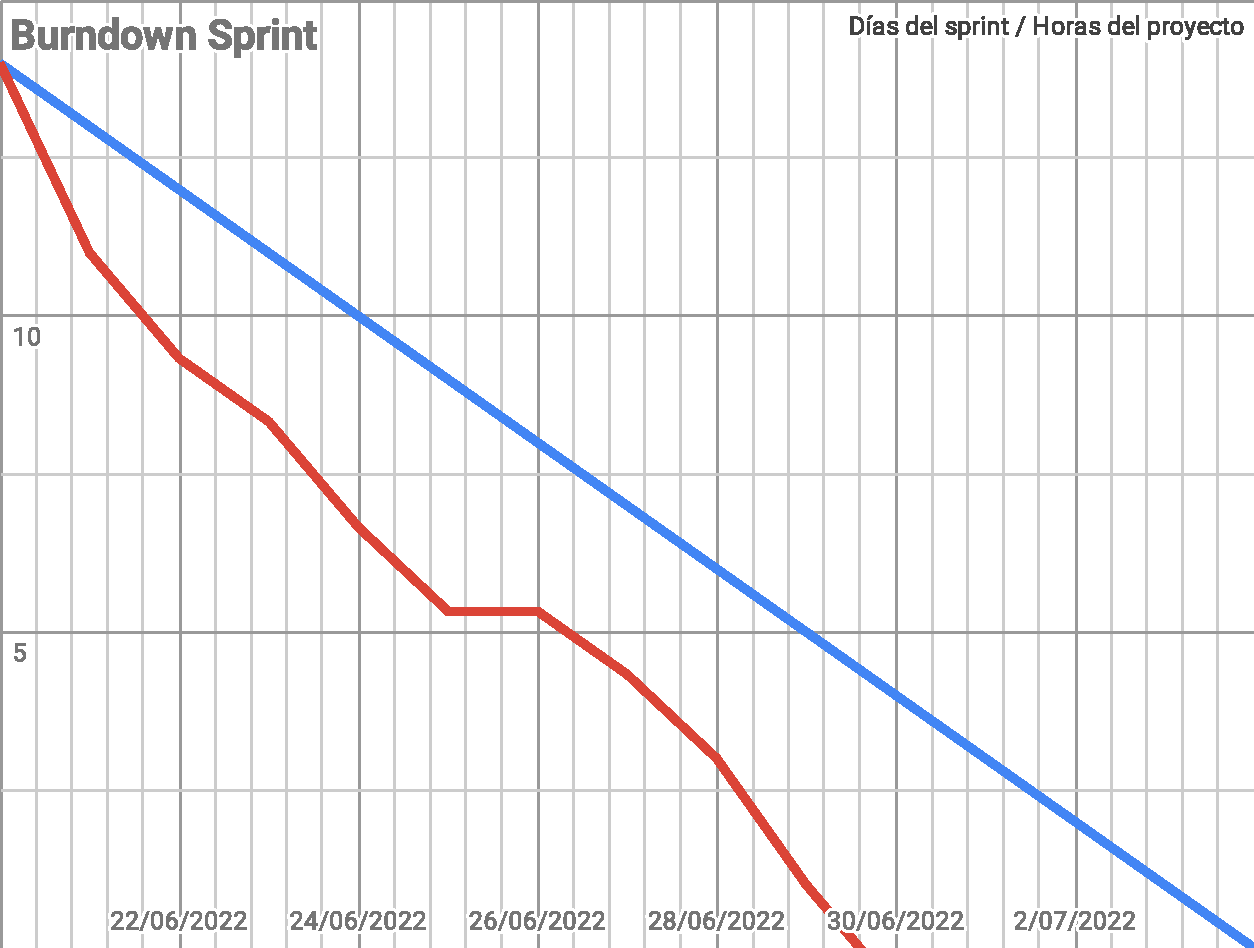
\includegraphics[width=1\linewidth]{text/image/BurndownChart7.pdf}
    \caption{Burndown chart $|$ Sprint 7 $|$ del 20/06 al 04/07}
    \label{fig:burndown_chart_7}
\end{figure}

\newpage
\paragraph{Sprint 8 (del 05/07 al 08/07)}
Este sprint posee una duración menor a las dos semanas habituales de sprints anteriores. Esto es debido a que es el último sprint del proyecto, el conocido como sprint de finalización. En este sprint el trabajo realizado va en relación a los últimos preparativos, correcciones y mejoras necesarios para cerrar y entregar el proyecto. Como se puede observar, se ha dedicado una cantidad mayor de horas que las que había planificadas.
\begin{figure}[H]
    \centering
    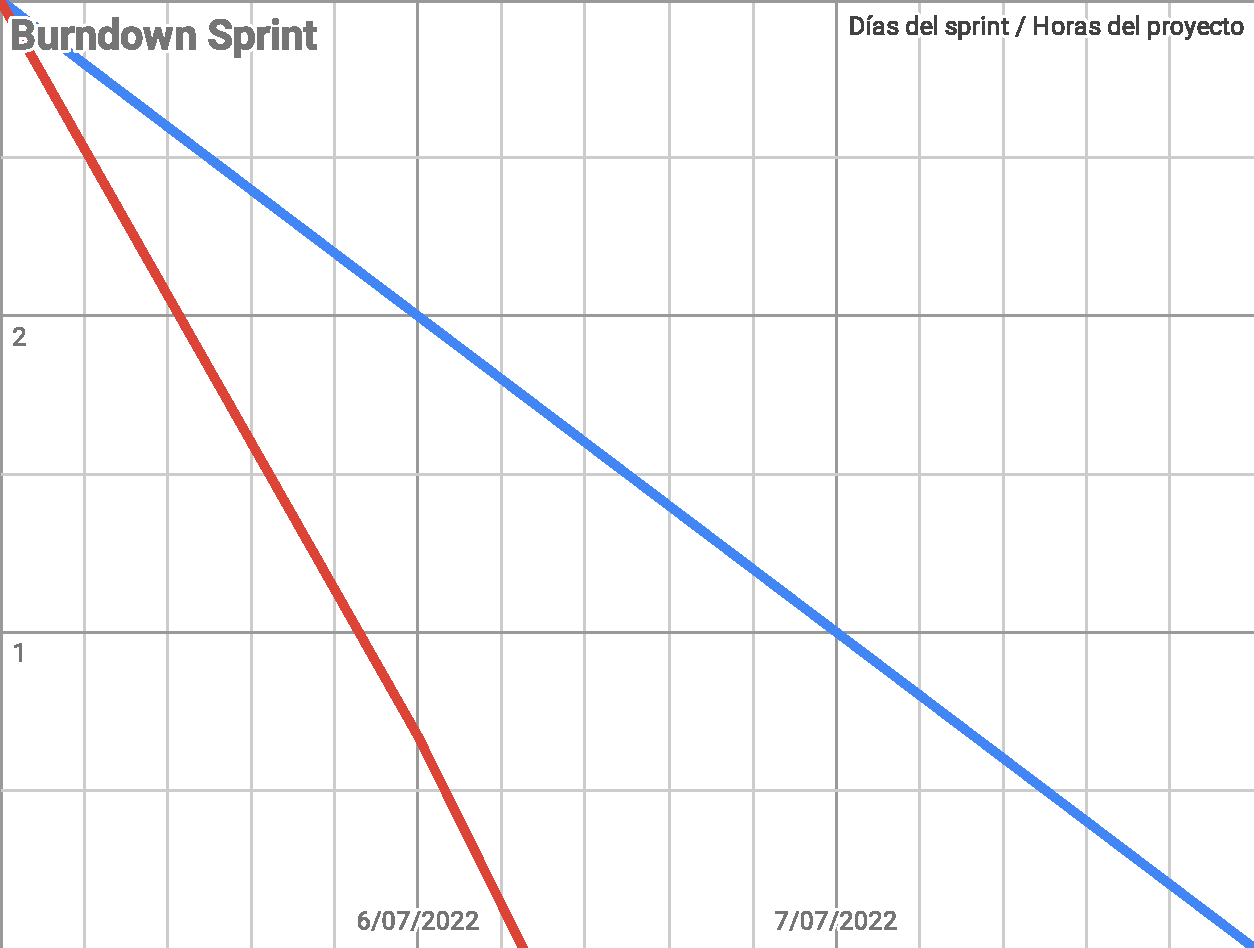
\includegraphics[width=1\linewidth]{text/image/BurndownChart8.pdf}
    \caption{Burndown chart $|$ Sprint 8 $|$ del 05/07 al 08/07}
    \label{fig:burndown_chart_8}
\end{figure}